\documentclass[tikz,border=18pt]{standalone}
\usepackage[utf8]{inputenc}
\usepackage[T1]{fontenc}
\usepackage{amsmath,amssymb}
\usepackage{fontawesome5}
\usetikzlibrary{arrows.meta, positioning, calc, fit, backgrounds, shapes.geometric}

% Harmonized palette matching Figures 1--4
\definecolor{unhblue}{RGB}{0,114,178}
\definecolor{cooppink}{RGB}{204,121,167}
\definecolor{textmain}{RGB}{15,23,42}
\definecolor{textmuted}{RGB}{100,116,139}
\definecolor{gridline}{RGB}{226,232,240}
\definecolor{nullred}{RGB}{190,18,60}
\definecolor{borderlight}{RGB}{203,213,225}
% Gate-specific (colorblind-safe)
\definecolor{passgreen}{RGB}{0,158,115}     % Okabe-Ito bluish green
\definecolor{passfill}{RGB}{222,241,235}    % light green fill
\definecolor{failfill}{RGB}{254,226,226}    % light red fill
\definecolor{amberfill}{RGB}{255,237,200}   % light amber (feasibility-counted)
\definecolor{amberedge}{RGB}{180,110,0}

\begin{document}
\begin{tikzpicture}[
    font=\sffamily,
    >=Stealth,
    % Cell styles
    cell/.style={draw=borderlight, line width=0.6pt, rounded corners=2.5pt,
                 minimum width=1.55cm, minimum height=0.86cm,
                 inner sep=1pt, align=center, font=\sffamily\bfseries},
    pass/.style={cell, fill=passfill, text=passgreen},
    fail/.style={cell, fill=failfill, text=nullred},
    partial/.style={cell, fill=amberfill, text=amberedge},
    hdr/.style={cell, fill=white, font=\sffamily\small\bfseries, text=textmain,
                draw=textmuted, line width=0.7pt, minimum height=1.05cm, align=center},
    rowlbl/.style={anchor=east, font=\sffamily\small, text=textmain},
    sumcell/.style={cell, fill=gridline, font=\sffamily\footnotesize\bfseries, text=textmain,
                    minimum height=0.7cm},
    note/.style={font=\sffamily\scriptsize\itshape, text=textmuted, align=left},
]

% ==================== COLUMN HEADERS ====================
\node[hdr] at (0,0.95)  {Event\\$G^{E}$};
\node[hdr] at (1.85,0.95){Policy\\$G^{P}$};
\node[hdr] at (3.70,0.95){Customer\\$G^{C}{\geq}2$};
\node[hdr] at (5.55,0.95){Human\\coding $G^{R}$};
\node[hdr] at (7.75,0.95){Layer-\\complete};

% ==================== ROW LABELS ====================
\node[rowlbl] at (-1.05,0)    {Mr.\ Cooper};
\node[rowlbl] at (-1.05,-0.95){UnitedHealth};
\node[rowlbl] at (-1.05,-1.90){HealthEquity};
\node[rowlbl] at (-1.05,-2.85){loanDepot};
\node[rowlbl] at (-1.05,-3.80){Navient};
\node[rowlbl] at (-1.05,-4.75){Cencora};

% ==================== GATE CELLS ====================
% Row 1: Mr. Cooper  -> E pass, P pass, C pass, R fail, layer-complete 3/4 (amber)
\node[pass] at (0,0)    {\faCheck};
\node[pass] at (1.85,0) {\faCheck};
\node[pass] at (3.70,0) {\faCheck};
\node[fail] at (5.55,0) {\faTimes};
\node[partial] at (7.75,0) {3/4};

% Row 2: UnitedHealth -> E pass, P pass, C fail (10-Q only), R fail
\node[pass] at (0,-0.95)    {\faCheck};
\node[pass] at (1.85,-0.95) {\faCheck};
\node[fail] at (3.70,-0.95) {\faTimes};
\node[fail] at (5.55,-0.95) {\faTimes};
\node[fail] at (7.75,-0.95) {2/4};

% Row 3: HealthEquity -> E pass, P pass, C fail, R fail
\node[pass] at (0,-1.90)    {\faCheck};
\node[pass] at (1.85,-1.90) {\faCheck};
\node[fail] at (3.70,-1.90) {\faTimes};
\node[fail] at (5.55,-1.90) {\faTimes};
\node[fail] at (7.75,-1.90) {2/4};

% Row 4: loanDepot -> E pass, P pass, C fail (10-Q only at gate time), R fail
\node[pass] at (0,-2.85)    {\faCheck};
\node[pass] at (1.85,-2.85) {\faCheck};
\node[fail] at (3.70,-2.85) {\faTimes};
\node[fail] at (5.55,-2.85) {\faTimes};
\node[fail] at (7.75,-2.85) {2/4};

% Row 5: Navient -> E pass, P fail (insufficient post-event text), C fail (CFPB + weak 10-Q), R fail
\node[pass] at (0,-3.80)    {\faCheck};
\node[fail] at (1.85,-3.80) {\faTimes};
\node[fail] at (3.70,-3.80) {\faTimes};
\node[fail] at (5.55,-3.80) {\faTimes};
\node[fail] at (7.75,-3.80) {1/4};

% Row 6: Cencora -> E pass, P fail (rebrand), C fail, R fail
\node[pass] at (0,-4.75)    {\faCheck};
\node[fail] at (1.85,-4.75) {\faTimes};
\node[fail] at (3.70,-4.75) {\faTimes};
\node[fail] at (5.55,-4.75) {\faTimes};
\node[fail] at (7.75,-4.75) {1/4};

% ==================== SUMMARY ROW (firms passing each layer) ====================
\node[rowlbl, font=\sffamily\footnotesize\bfseries, text=textmuted] at (-1.05,-5.80) {Firms passing};
\node[sumcell] at (0,-5.80)    {6/6};
\node[sumcell] at (1.85,-5.80) {4/6};
\node[sumcell] at (3.70,-5.80) {1/6};
\node[sumcell] at (5.55,-5.80) {0/6};
\node[sumcell, fill=amberfill, text=amberedge] at (7.75,-5.80) {1/6*};

% ==================== PER-FIRM FOOTNOTES (right margin) ====================
\node[note, anchor=west] at (8.75,0)    {censor before merger};
\node[note, anchor=west] at (8.75,-0.95){parent/unit/host caveat};
\node[note, anchor=west] at (8.75,-1.90){vendor-side event};
\node[note, anchor=west] at (8.75,-2.85){10-Q only at gate time};
\node[note, anchor=west] at (8.75,-3.80){event too recent};
\node[note, anchor=west] at (8.75,-4.75){rebrand discontinuity};

% ==================== LEGEND ====================
\node[draw=borderlight, fill=white, line width=0.8pt, rounded corners=5pt,
      inner sep=5pt, font=\sffamily\scriptsize, anchor=north west, align=left]
      at (-3.4,-6.7) {
    \begin{tabular}{cl}
        \tikz\node[pass, minimum width=0.5cm, minimum height=0.5cm, font=\sffamily\tiny]{\faCheck}; &
            \textbf{Pass} -- layer satisfied \\[2pt]
        \tikz\node[fail, minimum width=0.5cm, minimum height=0.5cm, font=\sffamily\tiny]{\faTimes}; &
            \textbf{Fail} -- layer not satisfied \\[2pt]
        \tikz\node[partial, minimum width=0.5cm, minimum height=0.5cm, font=\sffamily\tiny]{3/4}; &
            \textbf{Feasibility-counted} -- $\geq$3 layers but $G^{R}$ absent \\[2pt]
        \multicolumn{2}{l}{\textit{*1/6 = Mr.\ Cooper counted as fully measured for}} \\
        \multicolumn{2}{l}{\textit{feasibility accounting; verdict remains BOUND ($G^{R}$ fails for all).}}
    \end{tabular}};

\end{tikzpicture}
\end{document}
